% =========================================================================
% ESWA submission -- APPLICATION-FRAMED version (re-frame, not the method twin)
% An intelligent decision-support system for radar electronic-warfare
% intelligence analysis. Method (answer-geometry mismatch + typed operators)
% is the engine; the contribution is the deployed, auditable system.
% Compile: xelatex eswa; bibtex eswa; xelatex eswa; xelatex eswa
% =========================================================================
\PassOptionsToPackage{hidelinks}{hyperref}
\documentclass[review]{elsarticle}
\journal{Expert Systems with Applications}

\usepackage[T1]{fontenc}
\usepackage{microtype}
\usepackage{graphicx}
\usepackage{booktabs}
\usepackage{amsmath,amssymb}
\usepackage{array}
\usepackage{makecell}
\usepackage{multirow}
\usepackage{xcolor}
\usepackage{enumitem}
\usepackage{hyperref}
\usepackage{pifont}
\usepackage{tikz}
\usetikzlibrary{positioning,arrows.meta,fit,backgrounds,shapes.geometric}
\newcommand{\cmark}{\ding{51}}
\newcommand{\xmark}{\ding{55}}

% Chinese support (KG values are mixed Chinese-English)
\usepackage{xeCJK}
\IfFontExistsTF{SimSun}{%
  \setCJKmainfont{SimSun}\setCJKsansfont{SimSun}\setCJKmonofont{SimSun}%
}{\IfFontExistsTF{Noto Serif CJK SC}{%
  \setCJKmainfont{Noto Serif CJK SC}\setCJKsansfont{Noto Serif CJK SC}%
  \setCJKmonofont{Noto Serif CJK SC}}{}}

\usepackage{xurl}
\sloppy
\renewcommand{\arraystretch}{1.05}
\newcommand{\qtype}[1]{\texttt{\small #1}}
\newcommand{\op}[1]{\textsc{\small #1}}

\begin{document}

\begin{frontmatter}

\title{A Strategy-Routed, Auditable Decision-Support System for Radar
Electronic-Warfare Intelligence Analysis}

\author{Author Name}
\affiliation{organization={Your Institution}, country={China}}

\begin{abstract}
Radar electronic-warfare (EW) intelligence analysts must answer complex
questions over fragmented threat data --- enumerate every emitter a platform
carries, intersect several operating constraints, confirm the \emph{absence}
of a capability, or recommend countermeasures against a hostile air-defense
radar. In these settings an incomplete or wrong answer carries operational
cost, and the analyst must be able to trace every claim back to its source.
We present an intelligent decision-support system for radar EW intelligence
analysis, built on a curated radar knowledge graph (RadarKG-v2; 4{,}827
entities, 16{,}513 triples). Its retrieval engine departs from the top-$K$
paradigm underlying current GraphRAG: we show that top-$K$ embeds an
\emph{answer-geometry} assumption that fails systematically on enumeration,
intersection and complement queries, and replace it with a typed suite of six
retrieval operators, each derived from the information requirement of a query
class and selected by a lightweight large-language-model dispatcher. A
plan--execute--verify agent decomposes multi-step analyst requests while
keeping the language model \emph{out of the trust path}: every fact and number
is produced by deterministic knowledge-graph operators and reported with its
source and confidence. A doctrine-grounded module turns an enemy order of
battle into auditable countermeasure recommendations through weighted
set-cover wargaming. On a released bilingual benchmark of 499 questions the
system reaches \textbf{88.6\%} accuracy versus 52.7\% for a strong baseline
($+35.9$ pp), at \textbf{\$0.00041 per query}, and its typology transfers to a
general-domain knowledge graph without retraining.
\end{abstract}

\begin{keyword}
Intelligent decision-support system \sep Electronic warfare intelligence \sep
Knowledge graph question answering \sep Retrieval-augmented generation \sep
Auditable large-language-model systems
\end{keyword}

\end{frontmatter}

% =========================================================================
\section{Introduction}
\label{sec:intro}

\paragraph{The operational decision.}
A radar electronic-warfare (EW) intelligence analyst supports a recurring
decision: given a body of fragmented, multi-source threat data, characterize
an emitter or platform and, ultimately, recommend how to operate against it.
The questions that drive this decision are rarely single facts. They are
\emph{which} air-defense radars a particular system fields, \emph{how many}
emitters in a given band a platform carries, \emph{whether} a threat radar
has a stated home-on-jam capability, or \emph{what} countermeasures defeat a
specific hostile radar and at what residual risk. In an operational setting an
\emph{incomplete} enumeration (one missed emitter) or a \emph{false} assurance
(a capability wrongly reported absent) is not a ranking error --- it has a
cost. Two requirements follow that an off-the-shelf question-answering tool
does not meet: answers must be \emph{complete and structurally correct} for
the class of question asked, and every claim must be \emph{auditable} to a
named source so an analyst can decide how far to trust it.

\paragraph{Why generic GraphRAG is operationally inadequate here.}
Knowledge-graph retrieval-augmented generation (GraphRAG)
\citep{edge2024graphrag,gutierrez2024hipporag,peng2025graphrag} has become the
standard way to ground a large language model (LLM) in structured domain
knowledge. Yet essentially all GraphRAG variants --- community summarization,
Personalized PageRank, LLM path templates, beam search
\citep{luo2024rog,sun2024tog,ma2025tog2} --- retrieve a top-$K$ set of
passages or triples ranked by surface relevance. Top-$K$ silently assumes the
answer is a \emph{small set rankable by relevance}. That assumption is exactly
wrong for the analyst's hardest questions: an exhaustive count is bounded by
$K$ but the answer set is not; a multi-constraint filter cannot be expressed
by ranking; a non-membership claim cannot be confirmed by retrieving present
facts. The failure is \emph{information-theoretic}, not a matter of a weak
model or too small a $K$ (we show adding budget $K{=}8\!\to\!20$ recovers only
$+2.4$ pp). A decision-support system for this domain therefore needs a
retrieval layer whose \emph{access pattern matches the question's answer
geometry}, plus an orchestration layer that an analyst can audit.

\paragraph{Contribution.}
We design, build and evaluate an intelligent decision-support system for radar
EW intelligence analysis. Its contributions, in the order an analyst meets
them, are:
\begin{enumerate}[leftmargin=1.4em,itemsep=2pt]
\item A \textbf{domain knowledge base} (RadarKG-v2) and a deployed
question-answering front end that an analyst queries in natural language
(Chinese or English).
\item A \textbf{strategy-routed retrieval engine} that replaces top-$K$ with a
typed suite of six operators, each derived from the information requirement of
a query class. This is the system's analytical core; it lifts end-to-end
accuracy from 52.7\% to 88.6\% on a released benchmark.
\item A \textbf{plan--execute--verify agent} that decomposes multi-step
requests and, crucially, keeps the LLM \emph{out of the trust path}: all facts
and numbers come from deterministic graph operators and are reported with a
source and a confidence tier, so the output is an \emph{auditable intelligence
report}, not free-form generation.
\item An \textbf{EW countermeasure decision-support module} that turns an enemy
order of battle into doctrine-grounded countermeasure recommendations via
weighted set-cover wargaming, again with per-recommendation provenance.
\item A \textbf{released bilingual benchmark} (RadarKG-QA-499) and an honest
operating-cost characterization (\$0.00041 per query), so the system's claims
are reproducible and its deployability is quantified.
\end{enumerate}

% =========================================================================
\section{System overview and the analyst's decision pipeline}
\label{sec:overview}

Figure~\ref{fig:decision} shows the system from the analyst's point of view.
A natural-language request enters a \emph{planner} that decides whether it is a
single query or a multi-step task. Each query is routed by a lightweight
\emph{dispatcher} to the typed retrieval operator whose access pattern matches
the question, and the operator is executed \emph{only against the knowledge
graph}. Results flow into a \emph{verifier} that checks for empty or
suspicious outputs and can trigger one round of re-planning (e.g.\ a web lookup
for a model the graph does not yet cover). The analyst receives a report in
which every line carries its source and confidence; from the same evidence the
EW module can produce a countermeasure recommendation. The LLM appears only as
the dispatcher, the planner, and a final \emph{wording} stage --- never as the
source of a fact or a number.

\begin{figure*}[t]
\centering
\resizebox{\linewidth}{!}{%
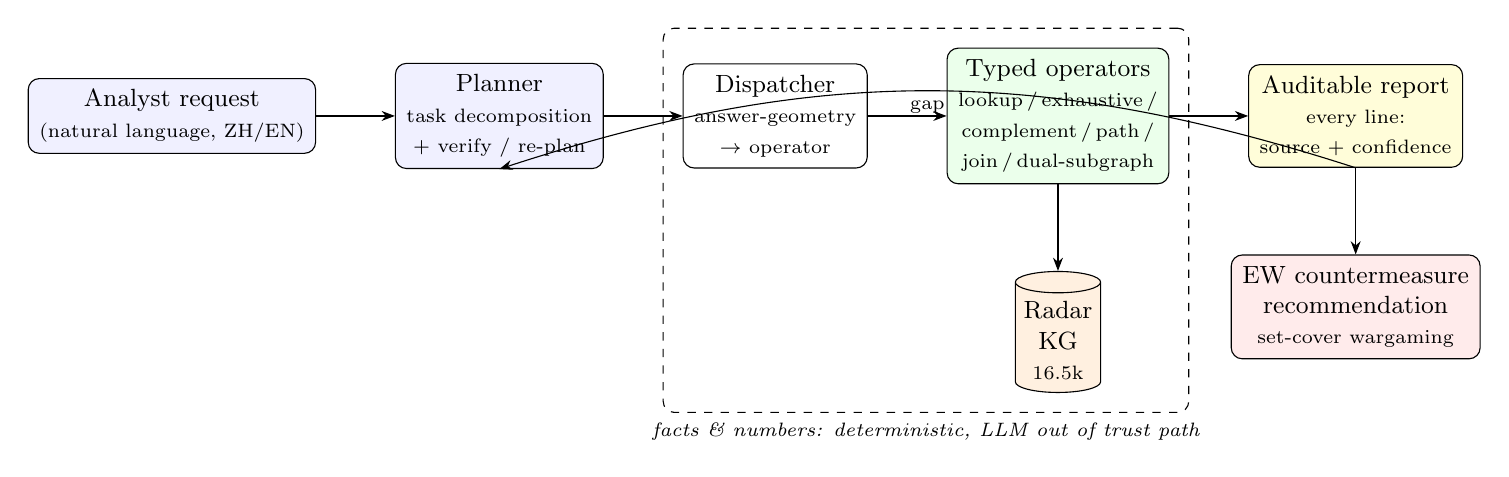
\begin{tikzpicture}[
  font=\small,
  node distance=7mm and 10mm,
  box/.style={draw,rounded corners,align=center,inner sep=4pt,minimum height=9mm},
  kg/.style={draw,cylinder,shape border rotate=90,aspect=0.25,align=center,inner sep=3pt},
  >={Stealth[]}]
\node[box,fill=blue!6] (q) {Analyst request\\\scriptsize(natural language, ZH/EN)};
\node[box,right=of q,fill=blue!6] (plan) {Planner\\\scriptsize task decomposition\\\scriptsize + verify / re-plan};
\node[box,right=of plan] (disp) {Dispatcher\\\scriptsize answer-geometry\\\scriptsize $\to$ operator};
\node[box,right=of disp,fill=green!8] (ops) {Typed operators\\\scriptsize lookup\,/\,exhaustive\,/\\\scriptsize complement\,/\,path\,/\\\scriptsize join\,/\,dual-subgraph};
\node[kg,below=11mm of ops,fill=orange!12] (kg) {Radar\\KG\\\scriptsize 16.5k};
\node[box,right=of ops,fill=yellow!15] (rep) {Auditable report\\\scriptsize every line:\\\scriptsize source + confidence};
\node[box,below=11mm of rep,fill=red!8] (ew) {EW countermeasure\\recommendation\\\scriptsize set-cover wargaming};
\draw[->] (q)--(plan); \draw[->] (plan)--(disp); \draw[->] (disp)--(ops);
\draw[->] (ops)--(kg); \draw[->] (ops)--(rep); \draw[->] (rep)--(ew);
\draw[->] (rep.south) to[bend right=18] node[midway,below,font=\scriptsize]{gap} (plan.south);
\begin{scope}[on background layer]
\node[draw,dashed,rounded corners,fit=(disp)(ops)(kg),inner sep=7pt,
  label=below:{\scriptsize\itshape facts \& numbers: deterministic, LLM out of trust path}]{};
\end{scope}
\end{tikzpicture}%
}
\caption{The analyst's decision pipeline. The language model serves as
planner, dispatcher and final wording only; every fact, count and absence
claim is produced by deterministic knowledge-graph operators and surfaced with
provenance. Figure~\ref{fig:pipeline} gives the internal stage view.}
\label{fig:decision}
\end{figure*}

% =========================================================================
\section{Knowledge base}
\label{sec:kg}

RadarKG-v2 has 4{,}827 entities and 12{,}219 inter-entity edges plus
${\sim}80$ typed numeric/categorical properties (16{,}513 triples total),
built from a 472-page airborne-radar handbook (full OCR), Wikidata SPARQL
pulls, and Wikipedia summaries. Country-of-origin and developer coverage are
93.4\% and 87.0\%. The schema is English; the value vocabulary is mixed
Chinese--English, reflecting how industrial defense KGs are actually
populated. Every triple carries a \texttt{source}, a \texttt{confidence}
score, and an \texttt{evidence} pointer; these metadata are what let the system
attach provenance to each answer line (\S\ref{sec:agent}). Numeric properties
are named \texttt{<property>\_<unit>} (e.g.\ \texttt{range\_km},
\texttt{peak\_power\_kW}); coverage of any single numeric property is partial
(${\sim}20$--$25\%$ of entities), so aggregate answers always report the
sample size $N/M$ rather than implying completeness.

% =========================================================================
\section{The retrieval engine: matching access pattern to answer geometry}
\label{sec:engine}

\subsection{Answer-geometry mismatch}
Top-$K$ retrieval is excellent for \emph{point} questions and structurally
wrong for \emph{aggregate} ones --- the same split databases draw between an
OLTP B-tree index and an OLAP scan \citep{codd1970relational}. Three query
patterns common in a threat KG break top-$K$ for distinct, computable reasons:
\textbf{unbounded enumeration} (the answer set can exceed any $K$),
\textbf{multi-constraint intersection} (ranking cannot express a logical AND),
and \textbf{complement / non-membership} (a KG stores positive facts, so an
absence is non-local). We call this the \emph{answer-geometry mismatch}: the
retrieval primitive's output shape does not match the shape of the answer the
question demands.

\subsection{A typed operator suite, derived not curated}
Rather than patch failures case by case, we enumerate the
information-requirement classes top-$K$ cannot satisfy and derive one operator
for each, adding \op{lookup} for the class top-$K$ \emph{does} satisfy
(Table~\ref{tab:reqs}). Each operator is the \emph{minimal} access pattern
meeting its row's requirement. Eleven analyst-facing question types map
deterministically onto the six operators (Table~\ref{tab:typology}). A
zero-shot LLM dispatcher (routing accuracy 93.0\%) reads the question and
selects the operator; a five-stage \textbf{bilingual alias layer} (direct
match $\to$ 614-form alias index $\to$ frequency-band normalization $\to$
suffix stripping $\to$ equivalence-class union) reconciles the mixed-language
values that defeat naive graph lookups. Figure~\ref{fig:pipeline} shows the
internal stages.

\begin{table*}[t]
\centering\small
\caption{Information-requirement derivation of the operator suite. Each row
determines its operator by the minimal access pattern satisfying the
requirement; top-$K$ fails for a different reason in each row.}
\label{tab:reqs}
\setlength{\tabcolsep}{4pt}
\begin{tabular}{p{0.18\linewidth} p{0.27\linewidth} p{0.28\linewidth} p{0.20\linewidth}}
\toprule
\textbf{Pattern} & \textbf{Information requirement (minimal)} & \textbf{Why top-$K$ fails} & \textbf{Derived operator} \\
\midrule
Identity / factoid     & one best-matching triple                                 & (none --- top-$K$ satisfies this)                                & \op{lookup} = BM25 $\oplus$ vec $\oplus$ RRF \\
Unbounded enumeration  & \emph{complete} head/tail set for a relation             & $K$ is an upper bound; answer set is not                         & \op{exhaustive} = $\{h \mid (h,r,t)\!\in\!\text{KG}\}$ \\
Multi-constraint AND   & set intersection of $N$ relations' head sets             & ranking cannot express AND; conflates signals                    & \op{constrained-join} = $\bigcap_i \text{heads}(r_i,t_i)$ \\
Complement / absence   & complete \emph{known} set, then explicit gap             & KG stores only positive facts; absence is non-local              & \op{complement} = enumerate then verify \\
Composition $(k\!\geq\!2)$ & path through $k$ relations preserving hop structure & top-$K$ is flat; loses hop boundaries                            & \op{path-plan} = $\text{tails}_{r_1}\!\circ\!\dots\!\circ\!\text{tails}_{r_k}$ \\
Binary comparison      & \emph{both} sides' subgraphs explicit and aligned        & top-$K$ may starve one side; cannot align                        & \op{dual-subgraph} = parallel $\text{tails}(A,B)$ + set ops \\
\bottomrule
\end{tabular}
\end{table*}

\begin{table}[h]
\centering\small
\caption{Analyst question types $\to$ operator (11-way typology).}
\label{tab:typology}
\begin{tabular}{p{0.35\linewidth} p{0.25\linewidth} l}
\toprule
\textbf{Type} & \textbf{Signal} & \textbf{Operator} \\
\midrule
\qtype{single\_hop}                                                 & entity + attr     & \op{lookup} \\
\qtype{relation\_inverse,} \qtype{agg\_count,} \qtype{agg\_enum}    & unbounded enum    & \op{exhaustive} \\
\qtype{two\_hop\_bridge,} \qtype{three\_hop\_chain}                 & composition $k\!\geq\!2$ & \op{path-plan} \\
\qtype{attr\_filter}                                                & AND of constraints & \op{constrained-join} \\
\qtype{negation,} \qtype{unanswerable}                              & absence            & \op{complement} \\
\qtype{set\_compare}                                                & two entities       & \op{dual-subgraph} \\
\qtype{distractor}                                                  & disambiguation     & \op{lookup} \\
\bottomrule
\end{tabular}
\end{table}

\begin{figure}[h]
\centering
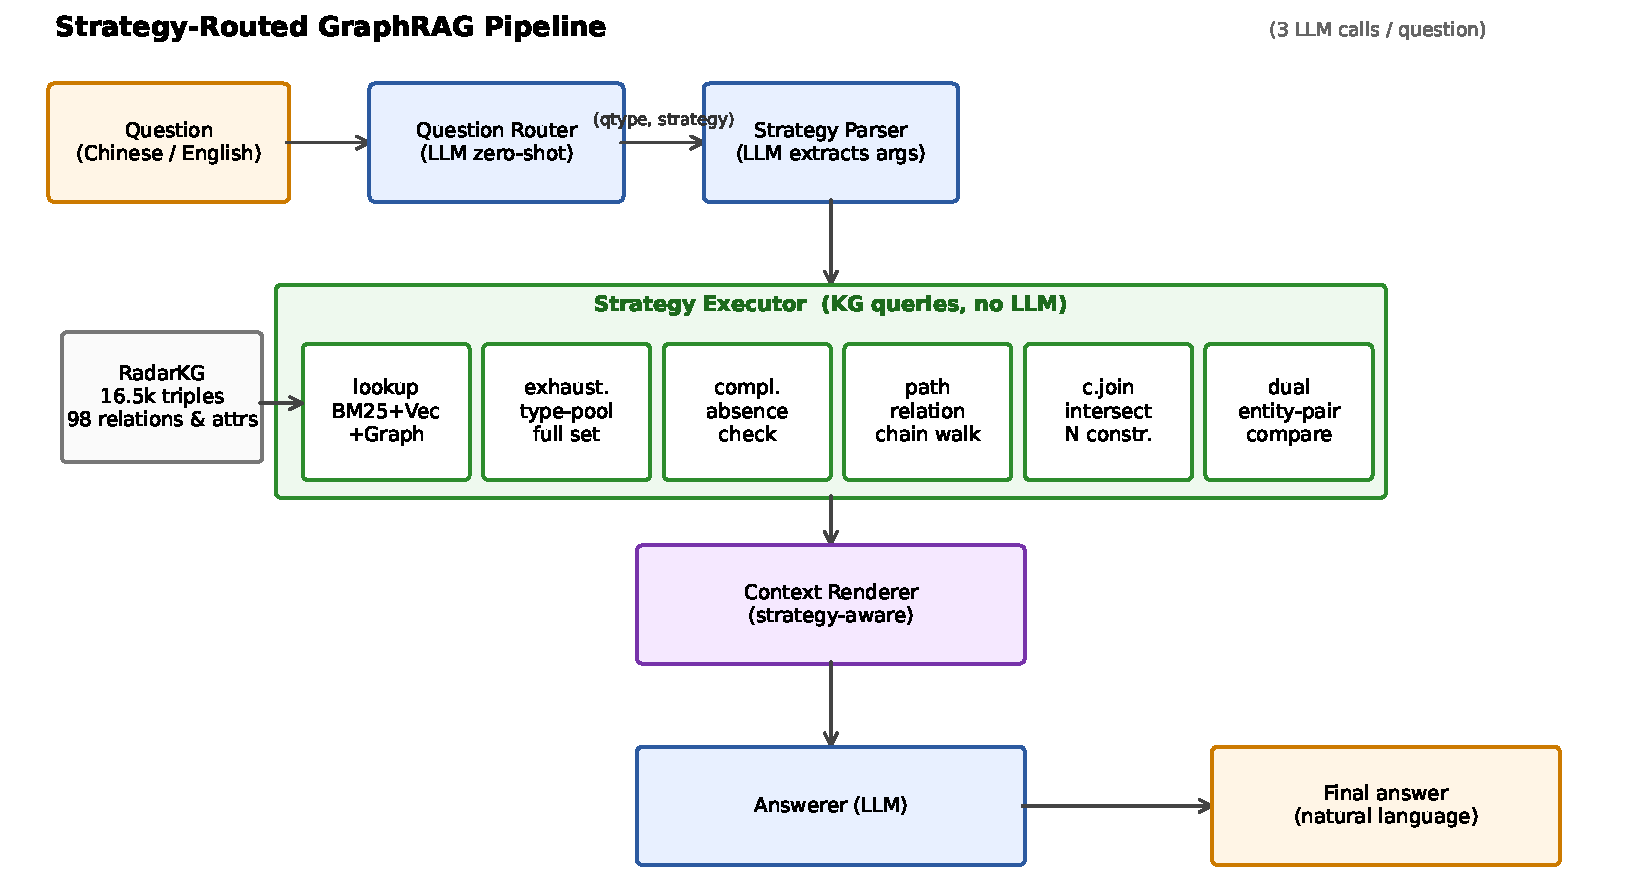
\includegraphics[width=0.95\linewidth]{figures/fig1_pipeline.pdf}
\caption{Internal stages of the retrieval engine: LLM dispatcher / parser /
answerer plus a KG-only executor. The KG is queried only in the executor.}
\label{fig:pipeline}
\end{figure}

% =========================================================================
\section{Agent orchestration and auditability}
\label{sec:agent}

Single queries rarely match an analyst's real request (``list this platform's
air-defense radars \emph{and} recommend a countermeasure for each''). A
plan--execute--verify agent handles such tasks. (i) A \emph{planner} LLM
decomposes the request into a step list with an explicit \emph{dataflow}: a
step argument may reference a previous step's result ($\$s_N$), and
\texttt{foreach}\,$\$s_N$ applies a tool to each item of a previous result set.
(ii) Steps are executed \emph{deterministically}; entity sets pass between
steps as values, never re-transcribed by the LLM, so nothing drifts. (iii) A
\emph{verifier} inspects the execution trace for deterministic gap signals
(empty set, ``not covered'', tool error, empty \texttt{foreach}); on a gap it
emits a revised plan once --- typically adding a web lookup for an
out-of-coverage model, or relaxing a constraint --- and re-runs.

\paragraph{The LLM is out of the trust path.}
This is the system's central design principle for a decision-support setting.
Every fact, count and absence claim in the output is produced by a
deterministic operator over the KG; the LLM only \emph{routes}, \emph{plans},
and \emph{phrases}. The intelligence report attaches to each conclusion the
\texttt{source} and \texttt{confidence} of the triples that produced it, and
the agent appends the deterministic artifact verbatim rather than letting the
LLM re-narrate it --- we observed that free-form final generation invents
parameters absent from the graph. Auditability is thus a structural property,
not a prompt instruction.

% =========================================================================
\section{Electronic-warfare countermeasure decision support}
\label{sec:ew}

The same provenance discipline drives the system's highest-value output: a
countermeasure recommendation against a hostile emitter. A \emph{doctrine
ontology} encodes jamming and electronic-counter-countermeasure (ECCM)
techniques and a \emph{defeats} relation $\mathcal{D}\subseteq E\times J$
between ECCM techniques $E$ and jamming techniques $J$, curated from
open-source EW doctrine
\citep{adamy2001ew101,schleher1999ew,zhang2023cognitiveew}. Given a threat
radar, the recommender returns a three-way verdict per technique ---
\emph{viable}, \emph{countered} (the radar fields a defeating ECCM), or
\emph{avoid} --- each tagged with the doctrine source and a confidence tier
(keyword match / LLM quote-verified / doctrine prior).

For a multi-emitter enemy order of battle the system frames countermeasure
selection as a \textbf{weighted set-cover} problem: choose a minimum-weight set
of jamming techniques that covers all threat emitters, solved greedily with the
classical $H_n\!\approx\!\ln n + 1$ approximation guarantee
\citep{chvatal1979setcover}. The output is an auditable wargaming plan: which
technique covers which threats, the residual uncovered set, and the doctrine
basis for each choice. This is a decision-support function in the strict sense
\citep{power2002dss} --- it structures and justifies a choice for a human
analyst, who retains the decision. The doctrine ontology comprises 17 jamming
techniques, 16 ECCM techniques and 14 recommendation rules; we evaluate its
fidelity and provenance in \S\ref{sec:eval-ew}.

% =========================================================================
\section{Evaluation}
\label{sec:eval}

\paragraph{Setup.} All systems use DeepSeek-Chat \citep{deepseekv3_2024}. We
compare three systems on all 499 benchmark questions: \textbf{Baseline} =
BM25 \citep{robertson2009bm25} + bi-encoder \citep{xiao2024bge} + reciprocal
rank fusion \citep{cormack2009rrf} + 2-hop expansion, top-$K{=}8$; a
\textbf{zero-shot path planner} (RoG-inspired \citep{luo2024rog}, single-policy
retrieval); and our \textbf{Strategy} engine. Confidence intervals are paired
bootstrap (1000 resamples). The comparator set is deliberately strong: the
path-planning baseline is Reasoning-on-Graphs (RoG) \citep{luo2024rog}, a
state-of-the-art reasoning-path GraphRAG method, evaluated both zero-shot and
--- as a \emph{supervised upper bound} --- faithfully LoRA-fine-tuned on two 7B
bases including RoG's original base (\S\ref{sec:related}); recent routing/tool
methods (Adaptive-RAG \citep{jeong2024adaptiverag}, ByoKG-RAG
\citep{byokgrag2025}) differ in kind, varying retrieval depth or source rather
than the primitive's semantics, and are discussed in \S\ref{sec:related}.

\subsection{The benchmark and why it is needed}
RadarKG-QA-499 contains 499 auto-generated, machine-verifiable questions
stratified across the 11 types, plus a 26-question out-of-distribution
bilingual stress subset that substitutes English/abbreviation aliases into
Chinese templates. Gold answers are computed directly from the KG's
ground-truth content (complete relation sets, true intersections, $k$-hop
terminal sets) \emph{independently of any system under test}; all three systems
recover the same target, so the comparison is fair and non-circular --- top-$K$
\emph{could} return a complete set but is structurally bounded by $K$ from doing
so, the phenomenon under study (that even our operators do not reach 100\% on
counting confirms the metric is not trivially satisfied). Correctness is exact
match (count equals gold count; set equals gold set), so the metric measures
\emph{fidelity to the KG}: residual KG noise sits in both the gold and any
faithful system's output and thus bounds absolute accuracy without affecting
the fairness of the comparison. The \op{constrained-join} equivalence-class
fallback (which unions the related \texttt{countryOfOrigin}/\texttt{operatedBy}
relations) is gated to fire only on an empty strict intersection and the gold
uses the strict relations; it fires on just 2 of 50 multi-constraint questions
and changes their accuracy by $0.0$ pp, so the multi-constraint gain is not an
artifact of relation loosening. We release it because \emph{no} public KGQA benchmark
stratifies for high-cardinality answer sets --- the cleanest signal of
retrieval-budget structural failure: RadarKG-QA-499 has $3.4\times$ the median
Count cardinality and $3\times$ the high-cardinality fraction of the
next-closest public benchmark (KQA Pro), and the same gap holds for
multi-constraint and three-hop questions (Fig.~\ref{fig:cardinality}). A system
meant to be \emph{trusted} on enumeration must be tested where enumeration is
hard.

\begin{figure}[h]
\centering
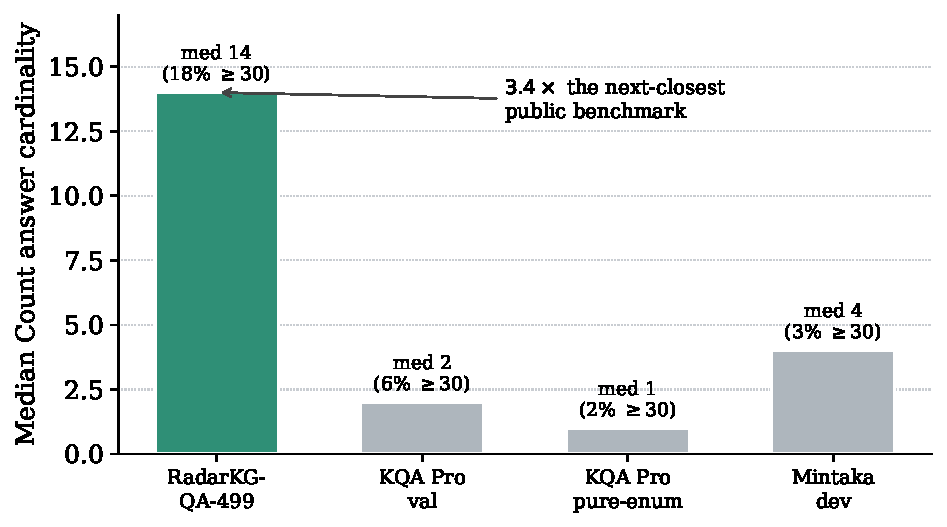
\includegraphics[width=0.82\linewidth]{figures/fig4_cardinality.pdf}
\caption{Count-question answer cardinality across benchmarks. RadarKG-QA-499
has $3.4\times$ the median and $3\times$ the high-cardinality ($\geq\!30$)
fraction of the next-closest public benchmark --- the regime where an analyst's
enumeration questions actually live.}
\label{fig:cardinality}
\end{figure}

\subsection{Decision-quality results}
The Strategy engine reaches \textbf{88.6\%} overall versus 52.7\% (Baseline)
and 60.3\% (path planner): $+35.9$ and $+28.3$ pp, with strictly positive
paired CIs and wins on 9/11 categories (Table~\ref{tab:main},
Fig.~\ref{fig:results}). The gains concentrate exactly where an analyst is
most exposed: $+58$ pp on counting emitters, $+80$ pp on multi-constraint
filtering, $+70$ pp on three-hop chains. Adding retrieval budget cannot
substitute: a $K{=}8\!\to\!20$ baseline gains only $+2.4$ pp, and Strategy
still leads the $K{=}20$ baseline by $+33.5$ pp --- because no $K$ bounds an
answer set that is structurally larger than $K$.

\begin{table*}[t]
\centering\small
\caption{Decision quality on RadarKG-QA-499 ($n{=}499$, accuracy \% with 95\%
paired bootstrap CI). Strategy wins on 9/11 categories with strictly positive
CIs.}
\label{tab:main}
\setlength{\tabcolsep}{3.5pt}
\begin{tabular}{l r l l l l l}
\toprule
\textbf{Type} & \textbf{n} & \textbf{Baseline} & \textbf{RoG} & \textbf{Strategy} & \textbf{$\Delta$ S$-$B} & \textbf{$\Delta$ S$-$RoG} \\
\midrule
\qtype{agg\_count}        & 50 & 4.0 [0, 10] & 38.0 [26, 50] & \textbf{62.0 [48, 74]} & $+$58 [$+$44, $+$72] & $+$24 [$+$12, $+$36] \\
\qtype{agg\_enum}         & 50 & 46.0 [32, 58] & 92.0 [84, 98] & \textbf{96.0 [90, 100]} & $+$50 [$+$36, $+$64] & $+$4 [$+$0, $+$10] \\
\qtype{attr\_filter}      & 50 & 12.0 [4, 22]  & 0.0           & \textbf{92.0 [84, 98]} & $+$80 [$+$66, $+$92] & $+$92 [$+$84, $+$98] \\
\qtype{relation\_inverse} & 50 & 40.0 [26, 54] & 74.0 [62, 86] & \textbf{86.0 [76, 94]} & $+$46 [$+$32, $+$60] & $+$12 [$+$4, $+$22] \\
\qtype{three\_hop\_chain} & 30 & 23.3 [10, 40] & 50.0 [33, 70] & \textbf{93.3 [83, 100]} & $+$70 [$+$53, $+$87] & $+$43 [$+$23, $+$63] \\
\qtype{two\_hop\_bridge}  & 80 & 40.0 [29, 51] & \textbf{95.0 [90, 99]} & 88.8 [81, 95] & $+$49 [$+$38, $+$60] & $-$6 [$-$14, $+$0] \\
\qtype{single\_hop}       & 80 & 83.8 [75, 91] & 11.2 [5, 19]  & \textbf{86.2 [79, 94]} & $+$2.5 [$+$0, $+$6] & $+$75 [$+$65, $+$85] \\
\qtype{set\_compare}      & 40 & 97.5 [93, 100] & 85.0 [73, 95] & 97.5 [93, 100] & 0 & $+$13 [$+$3, $+$23] \\
\qtype{negation}          & 40 & 100.0          & 97.5 [93, 100] & 100.0 & 0 & $+$3 [$+$0, $+$8] \\
\qtype{unanswerable}      & 20 & 90.0 [75, 100] & \textbf{100.0} & 90.0 [75, 100] & 0 & $-$10 [$-$25, $+$0] \\
\qtype{distractor}        & 9  & 100.0          & 66.7 [33, 100] & 100.0 & 0 & $+$33 [$+$0, $+$67] \\
\midrule
\textbf{OVERALL} & \textbf{499} & \textbf{52.7 [48, 57]} & \textbf{60.3 [56, 65]} & \textbf{88.6 [86, 91]} & \textbf{$+$35.9 [$+$32, $+$40]} & \textbf{$+$28.3 [$+$24, $+$33]} \\
\bottomrule
\end{tabular}
\end{table*}

\begin{figure}[h]
\centering
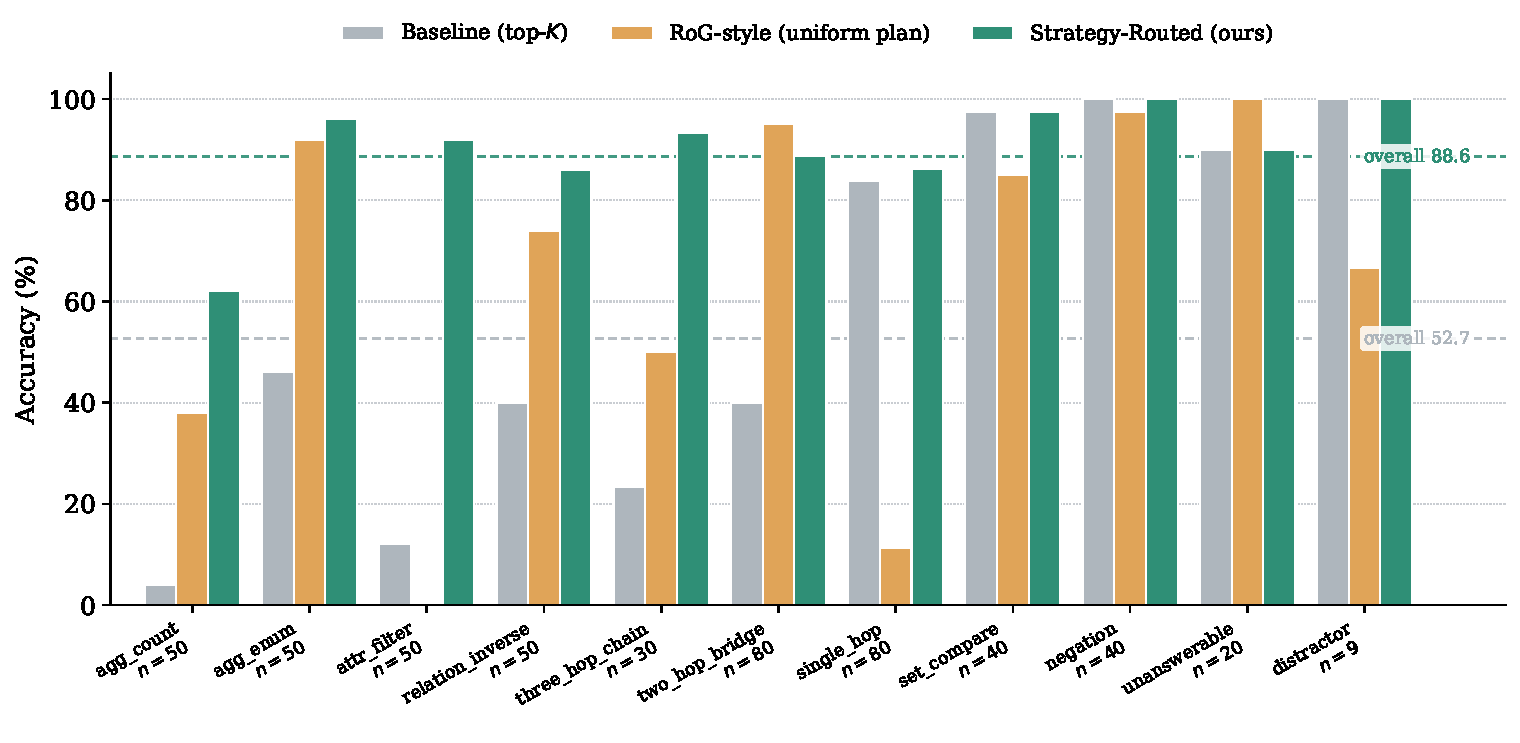
\includegraphics[width=0.98\linewidth]{figures/fig2_main_results.pdf}
\caption{Per-type accuracy: Baseline vs path planner vs Strategy. Gains
concentrate on the high-answer-geometry types (count, filter, multi-hop).}
\label{fig:results}
\end{figure}

\begin{figure}[h]
\centering
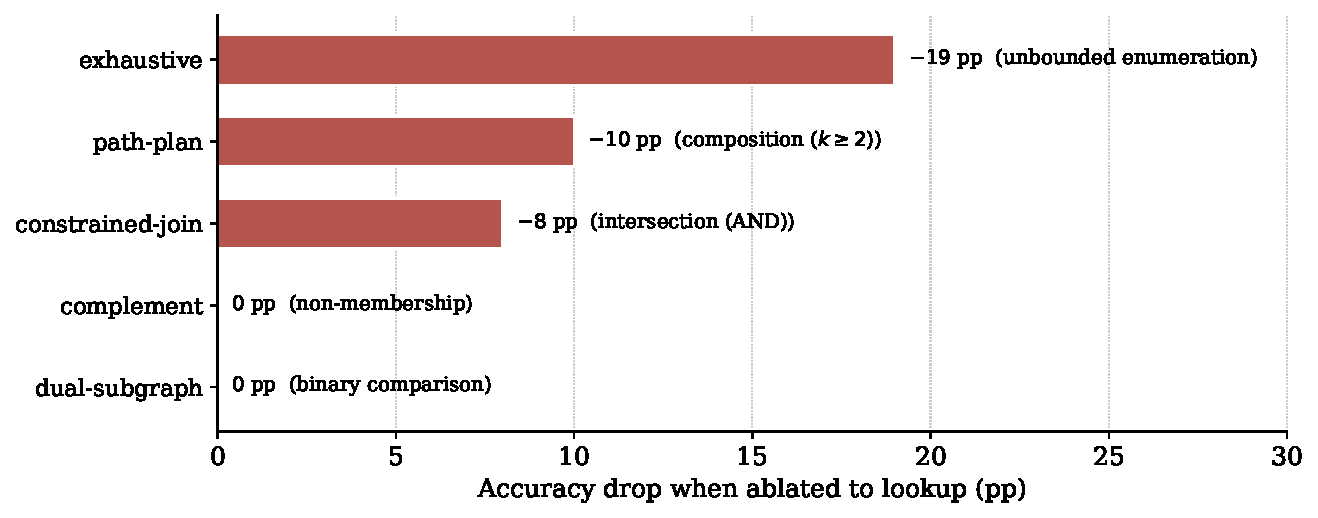
\includegraphics[width=0.92\linewidth]{figures/fig3_ablation.pdf}
\caption{Per-operator ablation: accuracy drop when each operator falls back to
\op{lookup}. Three load-bearing operators target disjoint answer-geometry
classes; \op{complement} and \op{dual-subgraph} read 0 pp on this benchmark's
negation/comparison distribution, not from redundancy.}
\label{fig:ablation}
\end{figure}

\subsection{Where the gain comes from}
An oracle-dispatcher ablation (gold question-type routing) reaches 88.2\% ---
within 0.4 pp of LLM dispatch (88.6\%) --- so the entire gain is
\emph{operator-driven}, not classifier luck. A per-operator ablation shows
three load-bearing operators on disjoint question slices (Fig.~\ref{fig:ablation}):
dropping \op{exhaustive} costs $-19$ pp, \op{path-plan} $-10$ pp,
\op{constrained-join} $-8$ pp ($-37$ pp total, accounting for the recoverable
failure budget). To
rule out a weak baseline, LoRA-fine-tuned path planners on two 7B bases
(including the original RoG base) improve ${\sim}{+}30$ pp over their zero-shot
selves yet still trail Strategy by $+27$ to $+33$ pp: a single-path planner
cannot express set-algebraic operators.

\subsection{Multi-step agent quality, cost, and transfer}
On a 72-task composition suite (six operator-composition classes, gold from the
deterministic executor) the agent achieves 100\% valid plans, 100\% execution,
and 99\% answer correctness --- the honest caveat being that this measures
planner quality against a deterministic ground-truth executor on
template-generated tasks. End-to-end cost is \textbf{\$0.00041 per query}
(\$0.00084 per accuracy point), well inside a deployable budget for an
analyst-facing tool. Finally, the typology and dispatcher transfer to
\textbf{KQA Pro} \citep{cao2022kqapro} (Wikidata) without retraining (67.4\%
zero-shot routing match; \op{dual-subgraph} $+11$ pp on SelectBetween),
evidence that the engine is not overfit to the radar domain. As a fully
external structural check, we also built a 19{,}540-triple Wikidata knowledge
graph (films domain) with SPARQL-computed gold --- neither the KB nor the gold
authored by us --- and 157 questions mirroring the answer-geometry types. On
the high-cardinality types (median gold cardinality 117) a generously
oracle-extracted top-$K{=}20$ baseline recovers 0--4\% while the typed operators
recover 100\%, with the single-hop control tied at 100\%: the structural gain
reproduces on an independent KB and gold (a deterministic, operator-level test).

\subsection{Countermeasure decision support: doctrine fidelity and provenance}
\label{sec:eval-ew}
The countermeasure module is evaluated on the two axes that matter for a
decision-support tool: is the advice doctrinally correct, and is every claim
auditable?

\paragraph{Doctrine fidelity.} On 16 hand-curated cases drawn from EW textbooks
--- \emph{independent} ground truth, not the engine's own rules --- the
advisor's recommendation includes the doctrinally correct technique and excludes
the wrong one in \textbf{16/16} cases (e.g.\ monopulse fire-control $\to$
cross-eye / cross-pol and \emph{not} inverse-gain; frequency-agile search $\to$
barrage / sweep and \emph{not} spot noise). Over all \textbf{650} threat
profiles the engine's invariants hold without exception (\textbf{0} violations):
a recommended technique is never simultaneously avoided or countered, every
cited doctrine rule resolves, and recommended equipment always band-matches the
threat. The knowledge base spans \textbf{89} SAM/IADS threat radars and
\textbf{4} documented historical SEAD engagements (Fan Song, Straight Flush, Low
Blow, Flat Face) used as independent sanity checks. End-to-end, an S-400 group
of five emitters is covered by a two-system equipment package (5/5 weighted
threats) with the SEAD priority correctly identified (the 92N6 engagement
radar).

\paragraph{Provenance / auditability.} Because facts never originate from the
LLM, auditability is measurable rather than asserted. Over 30 sampled
intelligence dossiers, \textbf{100\%} of deterministic facts (458/458) carry a
source and confidence, and the LLM executive summary is \textbf{100\%} grounded:
every entity and number token in the summary traces to a cited fact, with
\textbf{30/30} reports exhibiting zero fabrication. This quantifies the ``LLM
out of the trust path'' design of \S\ref{sec:agent}.

% =========================================================================
\section{Deployment considerations, trust, and limitations}
\label{sec:deploy}

\paragraph{Trust and failure cost.}
Because facts and numbers come only from deterministic operators, the failure
modes an analyst must guard against are bounded and legible: a missing edge in
the KG (surfaced as low coverage $N/M$, never silently completed), an
out-of-coverage model (surfaced as ``not covered'' and routed to a web lookup
flagged as unverified, confidence 0.6), or a dispatcher misroute (which
degrades gracefully to hybrid \op{lookup} rather than to a wrong operator's
empty set). No failure mode lets the LLM fabricate a parameter into a report.

\paragraph{Limitations.}
The system is a methodology and a research-grade testbed, not an accredited
operational tool: the KG is built from open and public-domain sources, so
absolute coverage of any real threat is limited by data access, not by the
method. The benchmark is auto-generated against the executor, so it measures
structural correctness rather than analyst-judged usefulness; a
human-in-the-loop study is future work. The six requirement classes are
grounded but not proven complete --- aggregation arithmetic, transitive
closure and temporal-range constraints would motivate further operators.

% =========================================================================
\section{Related work}
\label{sec:related}

\textbf{Knowledge-graph QA and GraphRAG.} Surveys \citep{peng2025graphrag} and
systems \citep{edge2024graphrag,gutierrez2024hipporag} ground LLMs in graphs;
reasoning-path methods
\citep{luo2024rog,sun2024tog,ma2025tog2,jiang2023structgpt} and KG-augmented
prompting \citep{baek2023kaping} all retrieve a relevance-ranked top-$K$ set.
\textbf{Adaptive retrieval.} Adaptive-RAG \citep{jeong2024adaptiverag} routes
by query \emph{complexity} and ByoKG-RAG \citep{byokgrag2025} fuses multiple
KG-retrieval tools, but both keep the retrieval primitive constant; we instead
vary the \emph{semantics} of the primitive (intersection vs enumeration vs
complement vs composition). \textbf{Cognitive EW decision support.} Radar
jamming decision-making \citep{zhang2023cognitiveew} and classical EW doctrine
\citep{adamy2001ew101,schleher1999ew} motivate the countermeasure module; our
contribution is to make the recommendation \emph{auditable} by grounding it in
a provenance-tagged KG and a set-cover formulation \citep{chvatal1979setcover}.

% =========================================================================
\section{Conclusion}
\label{sec:conclusion}

We presented an intelligent, auditable decision-support system for radar
electronic-warfare intelligence analysis. Its core insight --- that top-$K$
retrieval embeds an answer-geometry assumption that fails on the analyst's
hardest questions --- motivates a typed operator suite that lifts decision
quality from 52.7\% to 88.6\% while keeping the language model out of the trust
path, so every claim and every countermeasure recommendation is traceable to a
source. The system is deployable at \$0.00041 per query and its engine
transfers beyond the radar domain. We release the benchmark and knowledge graph
to support reproducible work on retrieval that matches the geometry of the
answer a decision actually requires.

% =========================================================================
\section*{CRediT authorship contribution statement}
\textbf{Author Name:} Conceptualization, Methodology, Software, Data curation, Formal analysis, Validation, Visualization, Writing -- original draft, Writing -- review \& editing.

\section*{Declaration of competing interest}
The authors declare that they have no known competing financial interests or personal relationships that could have appeared to influence the work reported in this paper.

\section*{Data availability}
The RadarKG-QA-499 benchmark, the RadarKG-v2 knowledge graph, and the evaluation and system code are openly available at \url{https://github.com/syx7597/radarkg-qa} and will be archived with a permanent DOI upon acceptance.

\section*{Funding}
This research received no specific grant from funding agencies in the public, commercial, or not-for-profit sectors.

\section*{Generative AI in the scientific writing process}
A large language model is a functional component of the proposed system (the dispatcher, planner, and answer-wording stages), as described in the manuscript. Separately, during manuscript preparation the authors used an AI assistant for language editing only; all scientific content was reviewed and verified by the authors, who take full responsibility for the publication.

\bibliographystyle{elsarticle-num-names}
\bibliography{references}

\end{document}
